\documentclass[report.tex]{subfiles}

\begin{document}
\section{Results and Discussion}

The FEM simulation was successful in outputting all parameters (figure \ref{fig:FinalSimulationResults}), showing that the OOF2 program can handle multi-grain images for the stress contour as well. The heat diffusion looks constant through the alpha and beta grains which is expected by their thermal conductivity values being similar. The x- and y- displacement contours are fairly consistent with previously generated results in the test cases, with the maximum displacement at 2.64 $\mu$m and 2.55 $\mu$m respectively. These displacement values are more similar than previous results, due to the image containing a more even quantity of alpha and beta and the coefficients of thermal expansion are more similar than the test cases.\\
\\ The stress contour shows a more interesting result which deviates from those found in test case 4. It shows that the stress of the alpha phase does not vary in the simulation and is close to 0 N/m$^2$, suggesting that the simulation has potentially only calculated the stress distribution in the beta phase. The stress in the beta region has the highest magnitude at the highest temperature and the magnitude gradually reduces with decreasing temperature. Unlike test case 4, the grain boundaries do not look to impact the stress distribution. It is clear from these unexpected results that significantly more research is required to understand how OOF2 creates the stress distribution contours and whether this is a reliable method to map stress in Ti-6Al-4V.

\begin{figure}[h!]
    \centering
    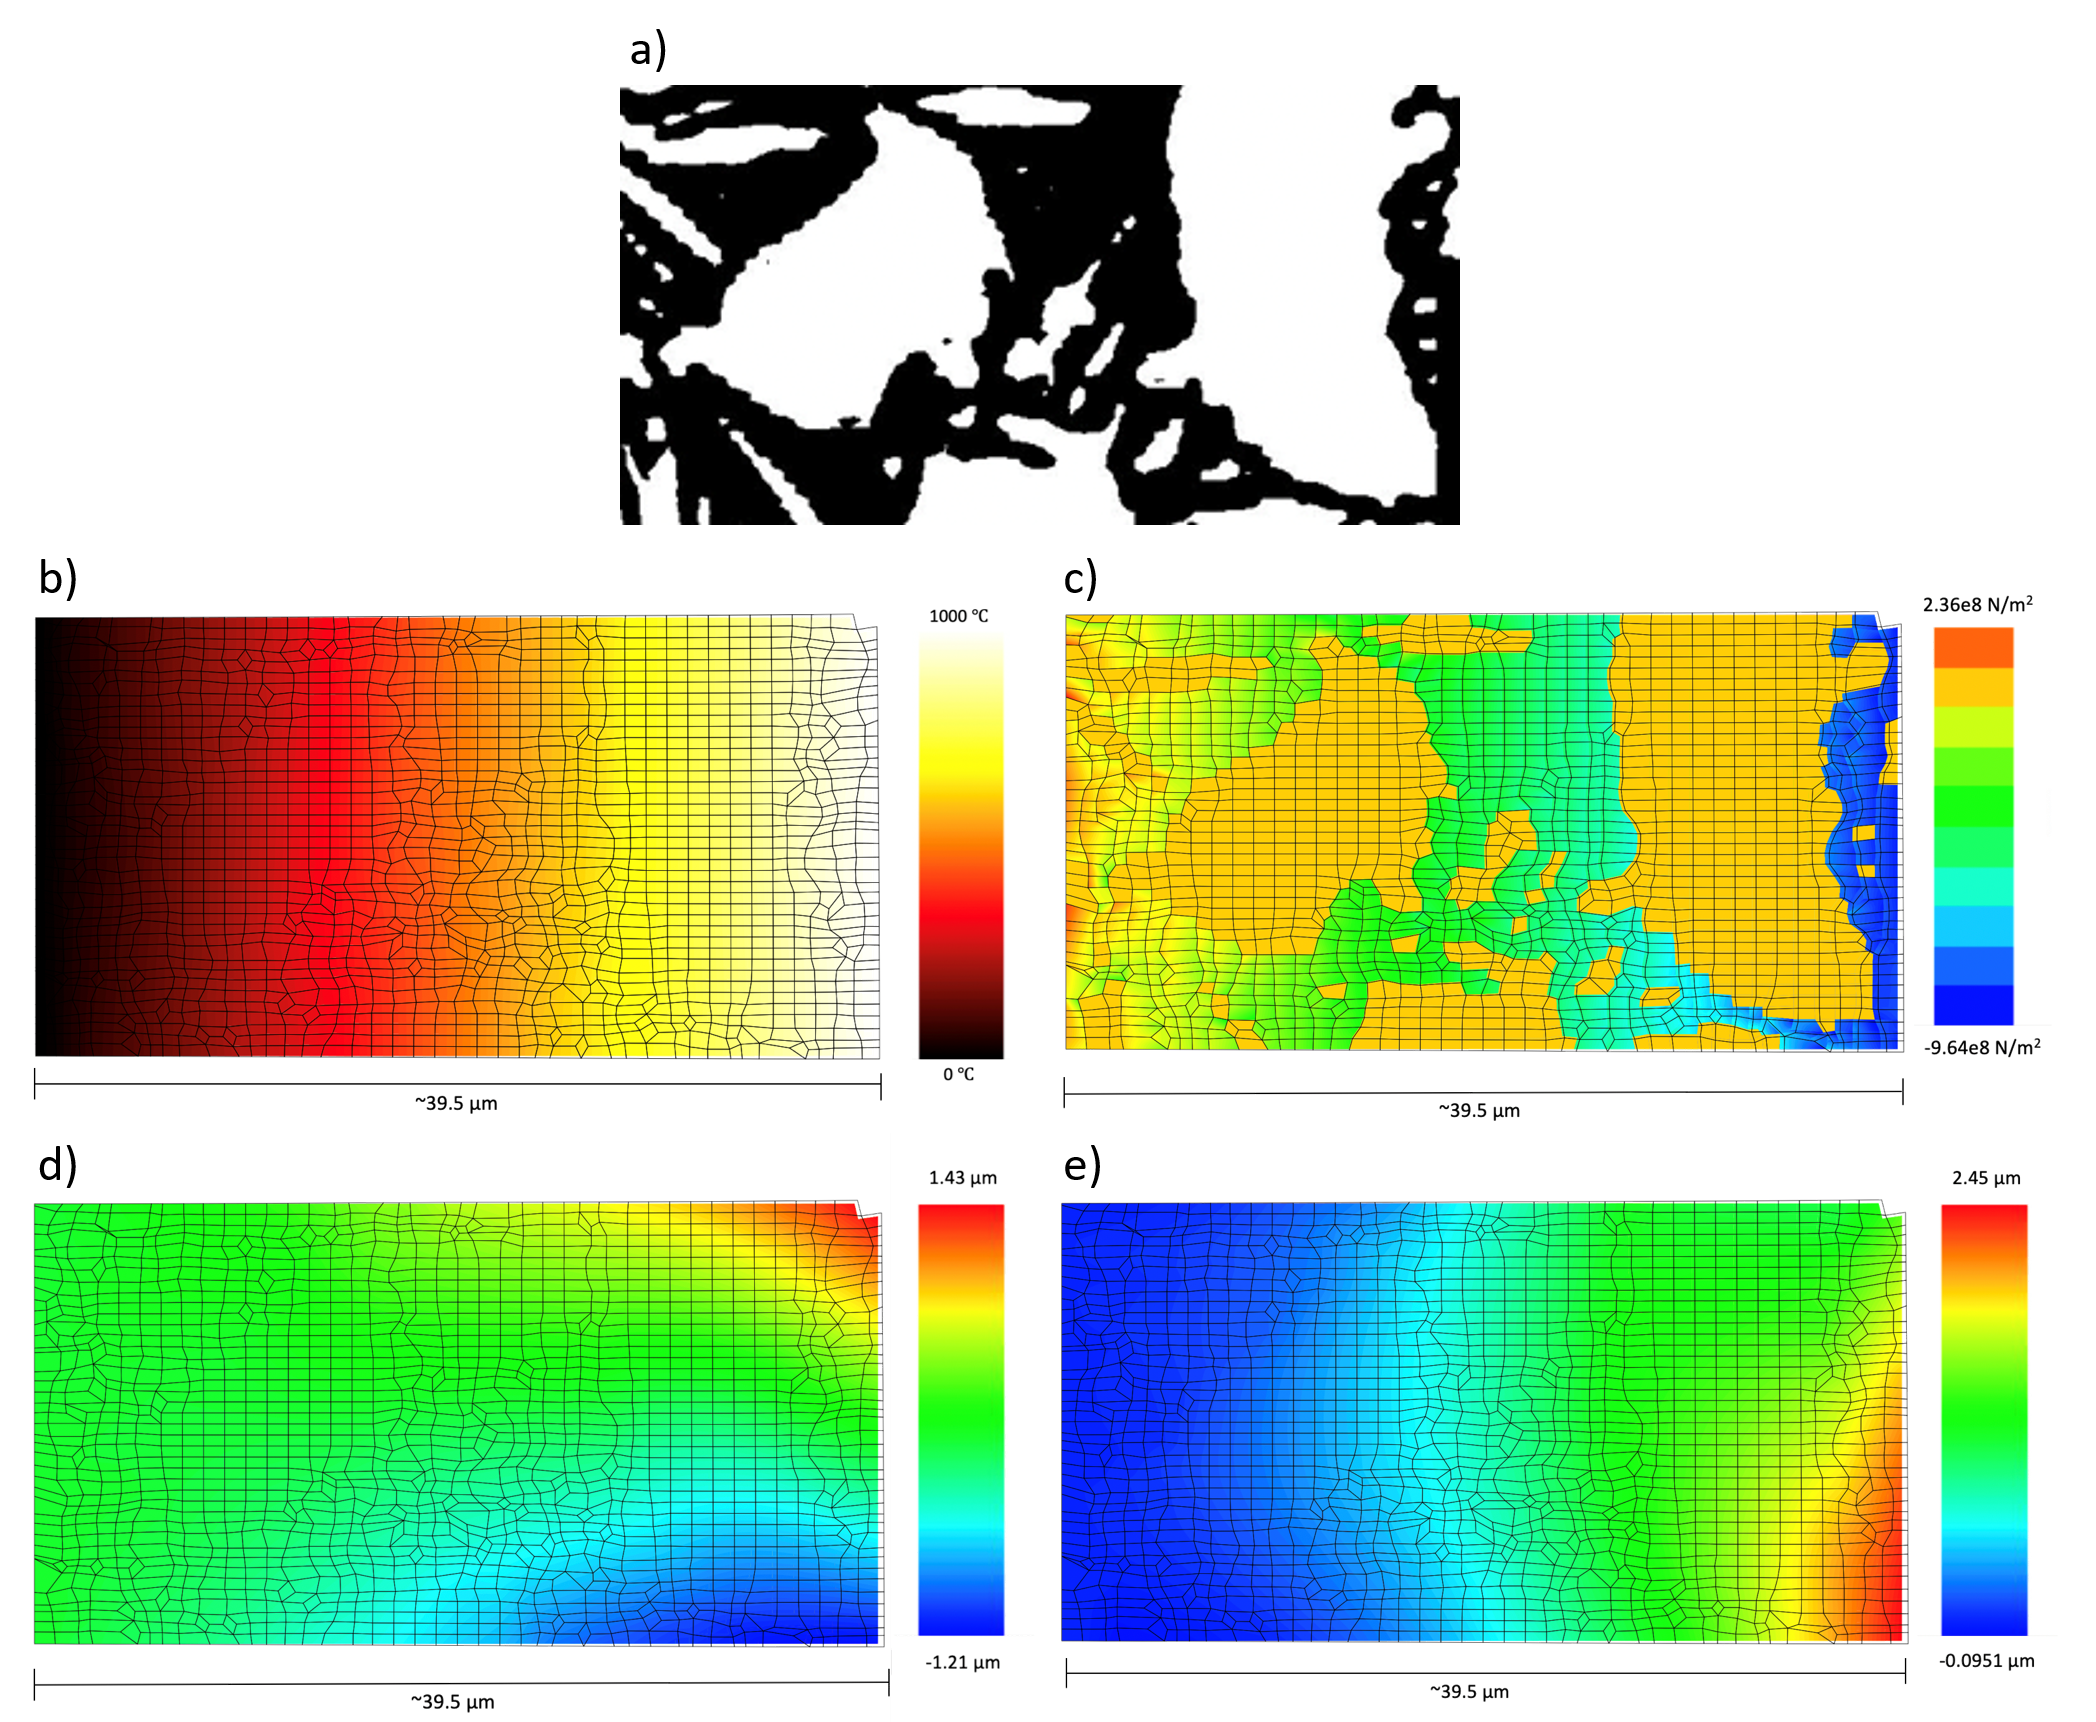
\includegraphics[width=17cm]{Ti64_Final_Simulation_Results.png}
    \caption{FEM simulation results, showing the a) original microstructure of Ti-6Al-4V b) heat diffusion through the grains c) stress    within the grains d) displacement in the x-direction e) displacement in y-direction}
    \label{fig:FinalSimulationResults}
\end{figure}


\end{document}
